\documentclass[a4paper,11pt]{article}
\usepackage{latexsym,amssymb,enumerate,amsmath,epsfig,amsthm}
\usepackage[margin=1in]{geometry}
\usepackage{setspace,color}
\usepackage{graphics}
\usepackage{subfigure}
\usepackage{relsize}
\usepackage{ifoddpage}
\usepackage{algorithmic}
\usepackage[ruled,vlined]{algorithm2e}

\usepackage[style=numeric, backend=biber, sorting=none]{biblatex}
\addbibresource{ref.bib}

%\newcommand{\x}{\mathbf{x}}
%\newcommand{\y}{\mathbf{y}}
%\newcommand{\bv}{\mathbf{v}}
%\newcommand{\n}{\mathbf{n}}
%\newcommand{\colored}[1]{\textcolor{red}{#1}}
%\newtheorem{thm}{Theorem}[section]
%\newtheorem{prop}{Proposition}[section]
%\newtheorem{obser}{Observation}[section]
%\newtheorem{corollary}{Corollary}[section]

%\doublespacing
\newcommand{\fro}[1]{\lVert #1 \rVert_F^2}
\newcommand{\nuc}[1]{\lVert #1 \rVert_*}
\newcommand{\norm}[2]{\lVert #1 \rVert_{#2}}
\newcommand{\half}{\frac{1}{2}}
\newcommand{\real}{\mathbb{R}}
\newcommand{\di}{\mathbf{d}_i}
\newcommand{\br}{\mathbf{r}}
\newcommand{\bd}{\mathbf{d}}
\newcommand{\be}{\mathbf{e}}
\newcommand{\bl}{\mathbf{l}}
\newcommand{\bx}{\mathbf{x}}
\newcommand{\by}{\mathbf{y}}
\newcommand{\bz}{\mathbf{z}}
\newcommand{\trace}{\text{tr}}
\title{Online Robust Principle Component Analysis With Huber Loss for Low-Rank
Image Recovery}
\author{
  Jacky Lau
}
\date{May 23, 2021}

\pagestyle{myheadings}

\begin{document}
\thispagestyle{plain}
\maketitle

%\begin{center}
%{\em Supervised by: } Dr. A-B-C 
%\end{center}
%\vspace{0.5cm}

\begin{abstract}
  \noindent Robust PCA (RPCA) and the recovery of low rank matrices have been
  studied extensively. While most RPCA algorithms rely on batch optimization,
  some online methods have since been proposed which are more computationally
  feasible for large datasets. In this report, we introduce a modified online
  RPCA method which uses the Huber loss function, as well as discuss some
  preliminary results on image inpainting and background separation.
\end{abstract}

\section{Introduction}
The topic of exact recovery of low-rank matrices has been widely studied with
many real work applications ranging from bioinformatics to image processing and
knowledge discovery. In recent years, many methods have been explored which
provide extensions to the singular value thresholding algorithm
\cite{cai2008singular} and the robust principle component analysis problem
\cite{NIPS2009}. One of the shortcomings of various robust PCA methods is that
these methods are generally based on batch optimization which requires the entire
set of sample data to be loaded into memory to perform SVD which can be
computationally infeasible for sufficiently large datasets. In \cite{FengORPCA},
an online implementation of principle component pursuit \cite{NIPS2009} using
stochastic optimization was proposed which can be applied to recover subspaces
of dynamic sample sets. This online robust PCA method is also able to handle
large scale datasets by revealing each sample sequentially and thus removing the
large memory requirement.

In this report, we will explore an extension of the online robust PCA method
using the Huber loss function \cite{Huber} with applications to image recovery.

\section{Online Robust PCA}
Suppose the data matrix $D \in \mathbb{R}^{m \times n}$, is generated by
corrupting a low rank matrix $A \in \mathbb{R}^{m \times n}$ with some sparse,
additive error $E \in \mathbb{R}^{m \times n}$, i.e., $D = A + E$. The robust
PCA problem \cite{NIPS2009} is to recover $A$ given $D$ such that
$A$ is low rank and $E$ is a sparse matrix which can be expressed as:
\begin{equation}
  \min_{A,\,E} \quad  \text{rank}(A) + \gamma \lVert
  \text{vec}(E)\rVert_0, \quad \textrm{s.t.} \quad D = A + E,
\end{equation}
where $\gamma$ is a Lagrangian multiplier. Considering the rank operator
and $\ell_0$  norm are non-convex functions, they can be substituted for their
respective convex surrogate functions, i.e., the nuclear norm and $\ell_1$ norm,
and expressed in the equivalent formulation:
\begin{equation}
  \min_{A,\,E} \quad \fro{D-A-E} + \lambda_1\nuc{A} + \lambda_2 \norm{\text{vec}(E)}{1}. 
\end{equation}

In \cite{FengORPCA}, in order to be able formulate the online optimization
problem, the rank of $A$ is upper bounded by $r$ such that $A$ can be
decomposed into the product of two matrices $L, R$ and the nuclear norm can be
expressed in the equivalent form \cite{Recht_2010}:
\begin{equation}
  \nuc{A} = \inf_{L \in \real^{p \times r}, R \in \real^{n \times r}}
  \left\{ \half \fro{L} + \half \fro{R} : A = LR^T\right\}.
\end{equation}
% TODO make sure dimensions are correct
% also make sure notation is consistent
Using this, the robust PCA problem can be reformulated as follows,
\begin{equation}
  \min_{L,R,E} \quad \fro{D-LR^T-E} + \frac{\lambda_1}{2}\left(\fro{L} + \fro{R}\right) 
  + \lambda_2 \norm{\text{vec}(E)}{1}. 
  \label{eqn:probl}
\end{equation}
Given a set of sample data $D = [d_1, \dots, d_n] \in \real^{p \times n}$,
\cite{FengORPCA} shows that minimizing the following cost function corresponds to the
optimal solution for problem \ref{eqn:probl},
\begin{equation}
  \label{eqn:cost}
  g_t (L) = \frac{1}{t} \sum_{i=1}^{t} \ell(\di) + \frac{\lambda_1}{2t} \fro{L}
\end{equation}
where $\ell$ denotes the loss function over each sample,
\begin{equation}
  \ell (\di, L) = \min_{\br, \be} \; \half \norm{\di - L\br - \be}{2}^2
   + \frac{\lambda_1}{2} \norm{\br}{2}^2 + \lambda_2 \norm{\be}{1}.
\end{equation}
The stochastic optimization algorithm for optimizing the cost function as
proposed in \cite{FengORPCA} is outlined in algorithm \ref{alg:orpca}, the
details of which regarding convergence guarantees are explained in the original
paper.

\vspace{5mm}

\begin{algorithm}[H]
  \caption{Online Robust PCA via Stochastic Optimization}
  \label{alg:orpca}
  \SetAlgoLined
  \KwIn{Observed data $\{\bd_1, \dots, \bd_T\}$, regularization parameters
  $\lambda_1, \lambda_2 > 0$, $L_0\in \real^{p \times r}$, $\br_0 \in \real^r,
  \be_0 \in \real^p$ }
  \For{$t = 1, \dots, T$}{
    Project new sample $\bd_t$:
    \begin{gather}
      \label{eqn:re}
      \{\br_i, \be_i \} \gets \arg \min_{\br, \be} \; \half \norm{\bd_t -
      L_{t-1}\br - \be}{2}^2 + \frac{\lambda_1}{2} \norm{\br}{2}^2 + \lambda_2
      \norm{\be}{1}.
    \end{gather}
    % TODO make change A and B, A is used to represent sparse matrix
    $Y_t \gets Y_{t-1} + \br_t \br_t^T,\; Z_t \gets Z_{t-1}+(\bd_t-\be_t)\br_t^T$ \\
    Update $L_t$ via algorithm \ref{basis}:
    \begin{gather}
      L_t \gets \arg \min_L \; \half \trace \left(L^T(Y_t+\lambda_1 I)L\right) - 
      \trace(L^T Z_t)
    \end{gather}
  }
  \Return $A = L_T R_T^T, \;E_T$
\end{algorithm}

\begin{algorithm}[H]
  \caption{Basis Update}
  \label{basis}
  \SetAlgoLined
  \KwIn{$L = [\bl_1, \dots, \bl_r ] \in \real^{p \times r},\; 
    Y = [\by_1, \dots, \by_r ] \in \real^{r \times r},\; 
    Z = [\bz_1, \dots, \bz_r ] \in \real^{p \times r},$ \\ $\tilde{Y} = Y+\lambda_1 I$.
  }
  \For{$j = 1, \dots, r$}{
    Update the $j$-th column vector of $L$:
    \begin{gather}
      \bl_j \gets \frac{1}{\tilde Y_{j,j}} (\bz_j - L\by_j) + \bl_j.
    \end{gather} 
  }
  \Return $L$.
\end{algorithm}

\section{OR-PCA with Huber Loss}
In this report we propose a modification to the online robust PCA algorithm 
which employs the Huber loss function \cite{Huber} as opposed to the squared
$\ell_2$ norm in \ref{eqn:re}. The Huber loss function is piecewise function given by,
\begin{gather}
  H_{\delta}(x) = 
  \begin{cases}
    \half x^2 & \text{for} \;|x| \leq \delta, \\
    \delta |x| - \half\delta^2  & \text{otherwise},
  \end{cases}
\end{gather}
which is quadratic for small values and linear otherwise which is commonly used
for introducing robustness to parameter estimation problems. For applying this
to the problem above, we use the sum of the elementwise Huber loss as the loss
function,
\begin{gather}
  F_\delta (\bx) = \sum_{i=1}^n H_\delta(x_i), \quad \bx \in \real^n.
\end{gather}
The modified algorithm is outlined below.

\vspace{5mm}

\begin{algorithm}[H]
  \caption{Online Robust PCA via Stochastic Optimization with Huber Loss}
  \label{orpca-huber}
  \SetAlgoLined
  \KwIn{Observed data $\{\bd_1, \dots, \bd_T\}$, regularization parameters
  $\lambda_1, \lambda_2 > 0$, $L_0\in \real^{p \times r}$, $\br_0 \in \real^r,
  \be_0 \in \real^p$ }
  \For{$t = 1, \dots, T$}{
    Project new sample $\bd_t$:
    \begin{gather}
      \{\br_i, \be_i \} \gets \arg \min_{\br, \be} \; F_{\delta}(\bd_t -
      L_{t-1}\br - \be) + \frac{\lambda_1}{2} \norm{\br}{2}^2 + \lambda_2
      \norm{\be}{1}.
    \end{gather}
    % TODO make change A and B, A is used to represent sparse matrix
    $Y_t \gets Y_{t-1} + \br_t \br_t^T,\; Z_t \gets Z_{t-1}+(\bd_t-\be_t)\br_t^T$ \\
    Update $L_t$ via algorithm \ref{basis}:
    \begin{gather*}
      L_t \gets \arg \min_L \; \half \trace \left(L^T(Y_t+\lambda_1 I)L\right) - 
      \trace(L^T Z_t)
    \end{gather*}
  }
  \Return $A = L_T R_T^T, \;E_T$
\end{algorithm}

\section{Results}
For the application of image recovery, we consider a series of images which are
similar but consisting of some corruption between each frame, for instance
foreground and background objects in a sequence of video frames or shadows in
face images. A set of sample images can be expressed as $D = [\bd_1, \dots,
\bd_n] \in \real^{hw \times n}$ where each column vector $\bd_i$ denotes the
flattened image with height $h$ and width $w$.

Figures \ref{fig:yale} to \ref{fig:badminton} show a comparison between the
recovered images using PCA/SVD, robust PCA \cite{NIPS2009}, online robust PCA
(ORPCA) \cite{FengORPCA}, and the proposed approach using the Huber loss
function. Figure \ref{fig:yale} shows the results on the Extended Yale Face
Database B \cite{cryale} with the recovered uncorrupted images and the
respective sparse error images, all the methods can somewhat successfully
subtract the shadows from the original face images; however, there is a slight
improvement in the quality using the Huber loss function over the regular
online RPCA method, RPCA and regular PCA.

Figure \ref{fig:security} shows the results on a set of roughly 100 frames of
stable security footage with similar results between the three robust methods
in terms of the quality of the recovered background images as well as the
sparse error. Figure \ref{fig:badminton} depicts a more prominent disparity
between the results of the four methods as the original images consisted of
camera jitter with quickly moving foreground elements. On this set of sample
images, the original RPCA method seems to produce the best result in terms of
the quality of the uncorrupted images while the other methods consisted of some
ghosting; however, the online RPCA methods produced the best results in terms
of the sparse noise components with the Huber loss providing some marginal
improvement.

Lastly, in figure \ref{fig:pattern}, we compare the results from inpainting a 
corrupted pattern image. In this case, we only use the single corrupted image 
as opposed to several stacked images as the underlying image contains a
consistent pattern which is low rank. The online RPCA method with the
Huber loss function is able to mostly recover the original image while
compromising slightly on some of the contrast and detail of the original image
while the other methods still contain a rather prominent darkened area where
the original corruption took place.

\begin{figure}[ht]
  \begin{center}
    \makebox[\textwidth][c]{
      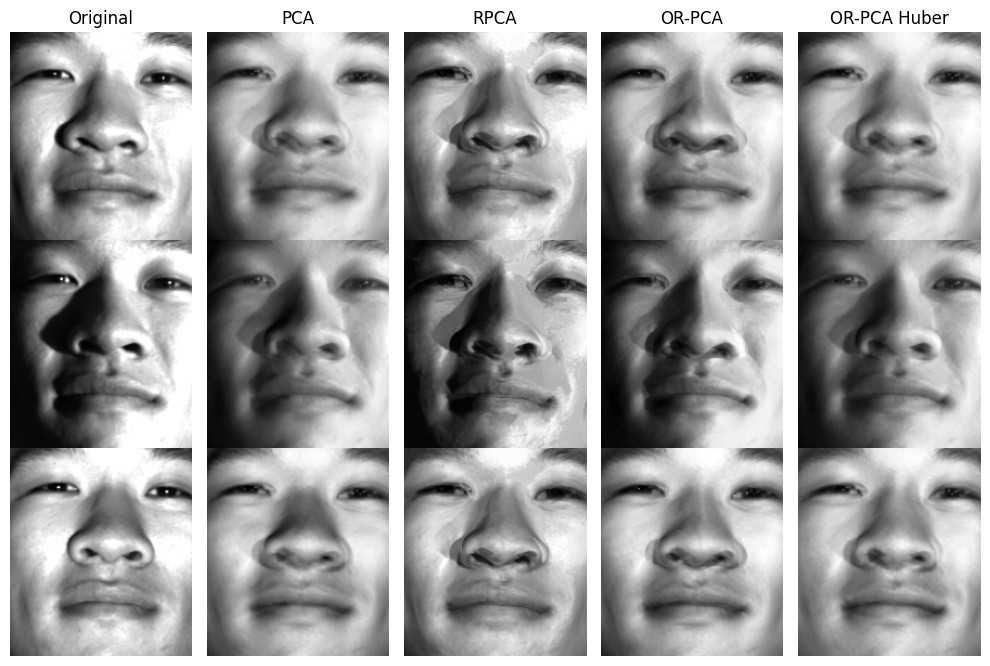
\includegraphics[width=0.55\linewidth]{cryale.png}
      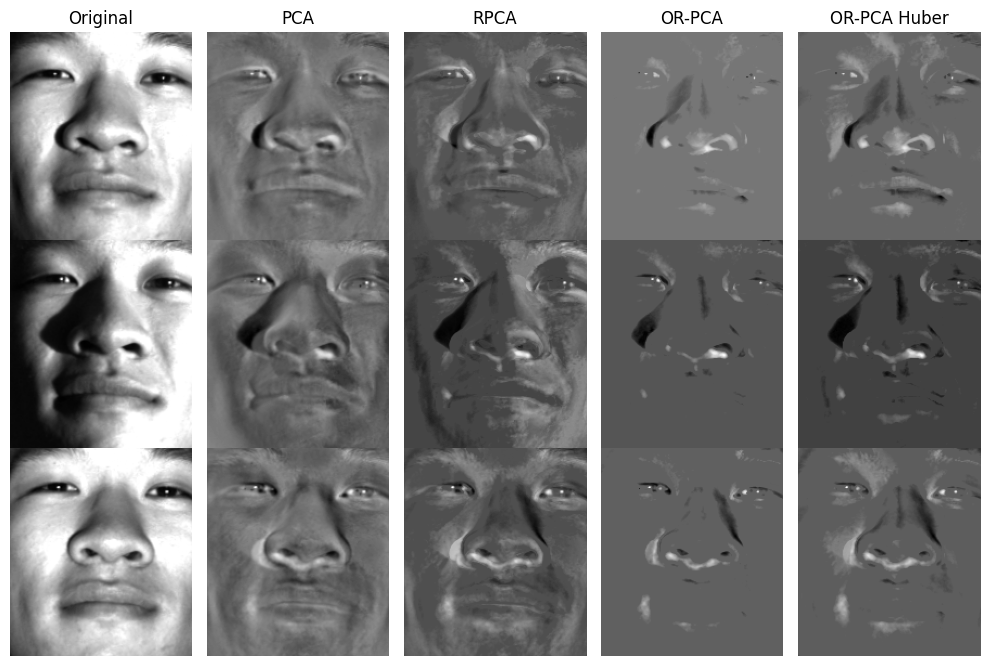
\includegraphics[width=0.55\linewidth]{cryale_noise.png}
    }
  \end{center}
  \caption{Face images from the Extended Yale Face Database B \cite{cryale}.}
  \label{fig:yale}
\end{figure}

\begin{figure}[ht]
  \begin{center}
    \makebox[\textwidth][c]{
    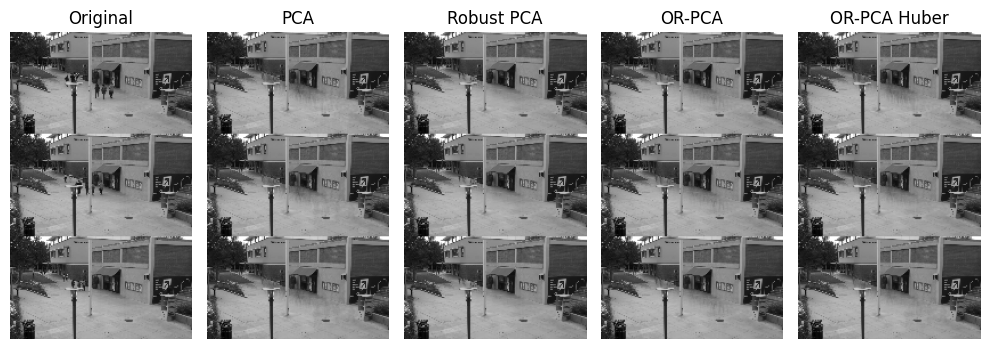
\includegraphics[width=0.55\linewidth]{security1.png}
    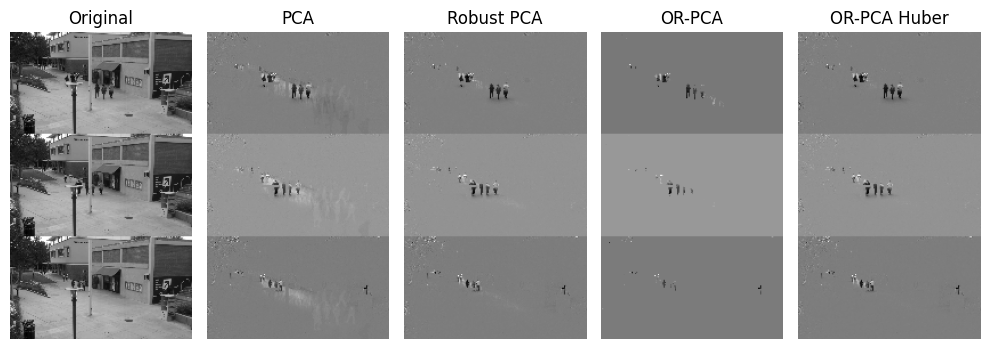
\includegraphics[width=0.55\linewidth]{security_noise1.png}
  }
  \end{center}
  \caption{Security footage.}
  \label{fig:security}
\end{figure}

\begin{figure}[ht]
  \begin{center}
    \makebox[\textwidth][c]{
    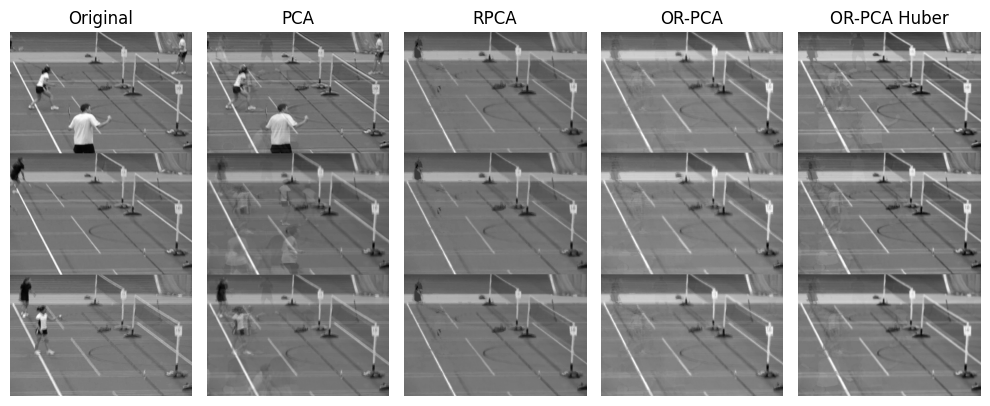
\includegraphics[width=0.55\linewidth]{badm.png}
    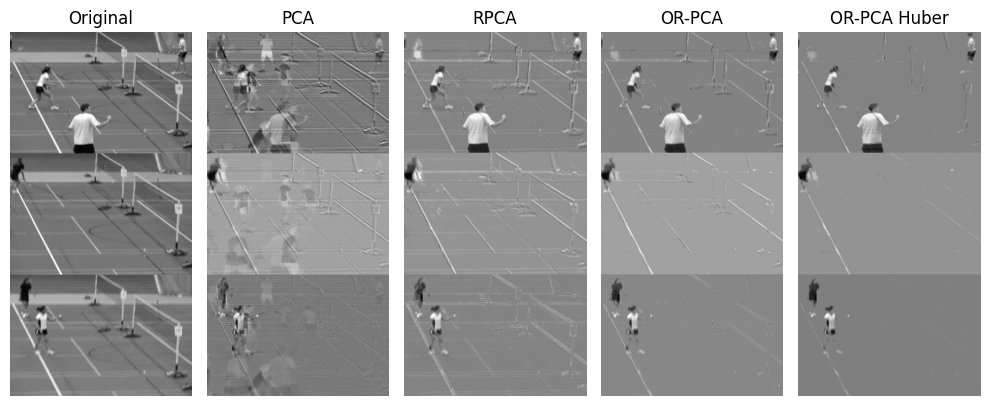
\includegraphics[width=0.55\linewidth]{badm_noise.png}
  }
  \end{center}
  \caption{Badminton footage with camera jitter from the ChangeDetection dataset
  \label{fig:badminton}
  \cite{changedetection}.}
\end{figure}

\begin{figure}[!htbp]
  \begin{center}
    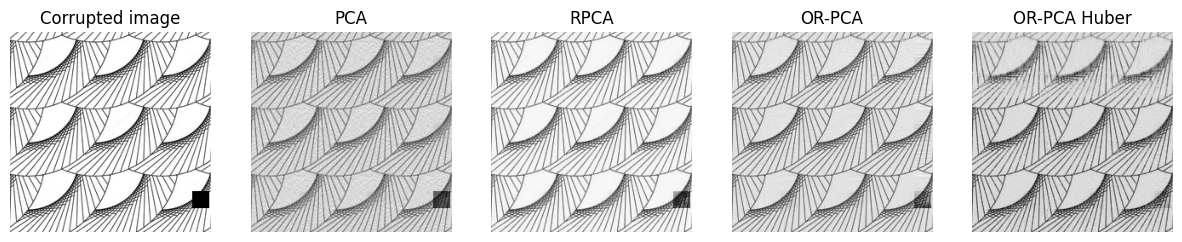
\includegraphics[width=\linewidth]{corupted_pattern.png}
  \end{center}
  \caption{Inpainting a corrupted pattern image.}
  \label{fig:pattern}
\end{figure}

\clearpage
\section{Conclusion}
In this report, we explored an extension of the online robust PCA method using
the Huber loss function which is more robust to large error terms. Empirically,
this modification to the original method is able to more appropriately separate the 
sparse error from a given set of samples, primarily in the context of
background-foreground subtraction as well as inpainting pattern images. Future
work may consider the theoretical properties of this modified loss on subspace
recovery.

\printbibliography
\end{document}
